\chapter{Objectives and Design}

This chapter will provide the overview of the goals set by the project, design implementation aimed to meet those and certain properties of the problem that affected the solution.
It will also cover design paradigms used for project guidance, as well as, the set of tools used for outlining its aspects.

\section{Main Objectives}

Throughout the course of project, the main aims that were targeted had been:

\begin{itemize}
\item {\textbf{Create a distributed version of NeMo, making it capable of scalable simulations with the use of multiple processes}}
\item {\textbf{Throughout implementation of the distributed capabilities, leave the core NeMo functionality intact - build on top}}
\item {\textbf{Implement clustering algorithm that would allow the resulting program to operate within the network capacity and distribute the workload in a more efficient manner}}
\item {\textbf{Lower the requirements set by the platform for the target machine(s) through parallelization}}
\end{itemize}

Setting out the objectives this way helped to percieve a more detailed picture of the project as a whole and gave understanding of the set of stages that were to be accomplished in order to
make the project meet these objectives.

\section{Objective-specific Structure}

After having all of the main goals set out, it is important to get the structure of the design, with focus on satisfying these goals. In this section, the design focused on each of the features of the project will be discussed.

\subsection{Distributed Version of the Simulator}

In order to provide a more detailed picture of the distributed system, here is the set of inner classes of the NeMo core simulation classes.

PICTURE

Creation of the distributed system that would run the simulator could be split into 3 distinct steps:

\begin{enumerate}

\item{\textbf{Creation of fully separate homogeneous simulation}}

By accomplishment of this step, the system has to be able to run on several processes with little input from the user and no interaction between processes within simulation - in other words, several separate NeMo simulations with their own self-generated parameters, that could be started by user signal from the main process.

\begin{figure}[h]
\begin{center}
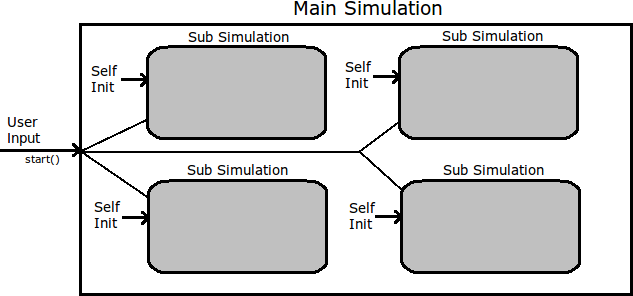
\includegraphics[scale = 0.25]{images/design_stage_1.png}
\end{center}
\caption{Schematic model of step 1}
\end{figure}

\item{\textbf{Integrating the initialisation parameters distribution across the network}}

After thorough research conducted into the use of MPI protocol, create a simulation that would encode and pass all the initialisation parameters to the networks - mapping, configuration, neuron and synapse data - however, still without interaction between the sub-simulations.

\begin{figure}[h]
\begin{center}
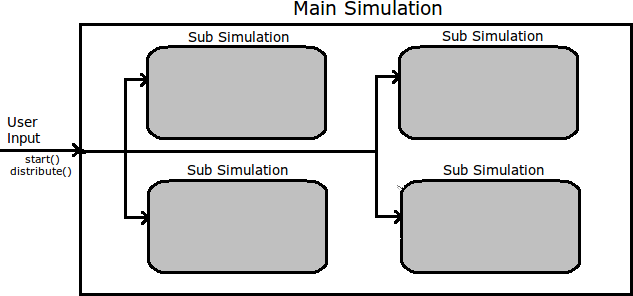
\includegraphics[scale = 0.25]{images/design_stage_2.png}
\end{center}
\caption{Schematic model of step 2}
\end{figure}

\item{\textbf{Implementation of the full non-constrained communication between the nodes within the network}}

Having the basic distribution system created, integrate the inter-node communication system that would allow subsystems to pass the internal spike data during simulations, while main class synchronizes the steps of all simulations by
waiting for all of the communication to end, and advancing simulation one step further.

\begin{figure}[h]
\begin{center}
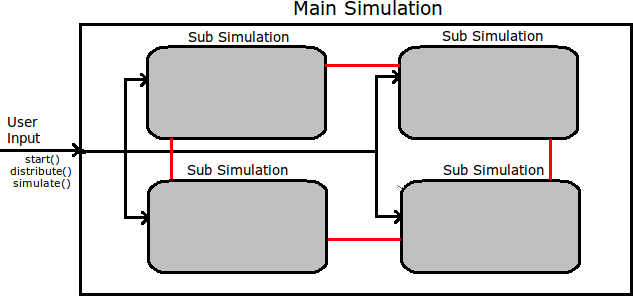
\includegraphics[scale = 0.25]{images/design_stage_3.png}
\end{center}
\caption{Schematic model of step 2}
\end{figure}

\end{enumerate}

Accomplishing all of these steps yields a fully working distributed implementation of the target system. It is worth noting that though this design is quite schematic, the results of the actual implementation if broken into steps were closely related to those presented by this plan.

\subsection{Separation from the Core System}

\begin{figure}[h]
\begin{center}

\includegraphics[scale = 0.1]{images/placeholder.jpg}
\end{center}
\caption{NeMo simulation core}
\end{figure}

These classes is the core of the NeMo functionality, as it comprises all the data sets needed for the correct simulation. Therefore, in order to enable the distributed version to run separately, i.e. without interfering with the data innate to these classes, it is essential to design the system around those. In other words, the correct design must not alter internal structure of this set of classes.

\begin{figure}[h]
\begin{center}

\includegraphics[scale = 0.1]{images/placeholder.jpg}
\end{center}
\caption{Distributed simulation design}
\end{figure}

As it can be easily observed, the distributed version treats the core simulation classes as separate entities, only interacting with them through the NeMo-specified functionality and set of public methods, already present in them.
Objectively, the MPI Layer wraps around the simulation classes and enables communication by passing input and output data between separate NeMo simulations.

\subsection{Mapping}

\begin{figure}[h]
\begin{center}

\includegraphics[scale = 0.1]{images/placeholder.jpg}
\end{center}
\caption{Mapping scheme}
\end{figure}

\subsection{Alternative Solutions}
\begin{itemize}

\item {Latency and Spike delivery}

Due to latency within the network of processors the system was tested on, there were a few precedents of race conditions that caused uncertain behaviour of the simulator - therefore, giving output that differed significantly from the desired one. In order to overcome this drawback, a timer system within the master simulation has been implemented - this ensured control of the communications, and allowed for stops with delay, to deal with propagating spikes. That move has significantly increased precision of the simulation, moreover, giving a better overview of the performance.

\end{itemize}


\section{Final Design}

\section{Tools}
